\documentclass[12pt]{article}
\usepackage{graphicx}

\title{Visualization and Analysis of Calcification Effects in Balanophyllia Europea Corals}
\author{Kristin Rieping (10252428) \and Toby Hijzen \and Mihai Morariu (10232710) \and Robrecht Jurriaans}
\date{}

\begin{document}

\maketitle

\begin{abstract}
In this report we describe the pipeline for the visualization of the calcification in balanophyllia europea corals. We also analyze, using the tools provided by the VTK visualization framework, the effects on calcification for corals grown in two different types of environments: acidified and non-acidified water. The data we are provided is in the form of DICOM 2D slices and was acquired using a CT scanner. We build a pipeline in which the data of a batch of corals is separated, visualized and analyzed.
\end{abstract}

\section{Introduction}

\

Coral reefs are among the oldest and most valuable ecosystems on Earth. According to the U.S. National Oceanic and Atmospheric Administration\footnote{http://oceanservice.noaa.gov/education/kits/corals/coral07\_importance.html}, they support more species per unit area than any other marine environment, including about 4000 species of fish, 800 species of hard corals and hundreds of other species. They also support a variety of human needs - for example, they are an important source of compounds for the development of drugs used as possible cures for cancer, arthritis, human bacterial infections, viruses and other diseases. For these reasons, careful preserving of coral reefs is important for keeping a long-term balance in the environment. 

\

One of the most critical effects of increasing ocean acidity relates to the production of shells, skeletons and plates from calcium carbonate (CaCO$_3$), known as \emph{calcification}. Acidification reduces the amount of carbonate ions that are available for corals and other marine calcifiers to build their skeletons. Since reef-building corals need carbonate to build them, decreasing carbonate ion concentrations will likely lead to weaker, more brittle coral skeletons and slower coral growth rates.

\

\subsection{Corals}

\

We are given two batches of 10 baranophyllia europea corals that were scanned using a CT scanner (figure \ref{fig:1}). The first batch was grown in a normal, unacidified water environment, while the second one was grown in acified water. We use the data in order to visualize the calcification in each coral sample, but also to analyze the effects of acidification on the calcium layers.

\

\begin{figure}[!h]
\centering
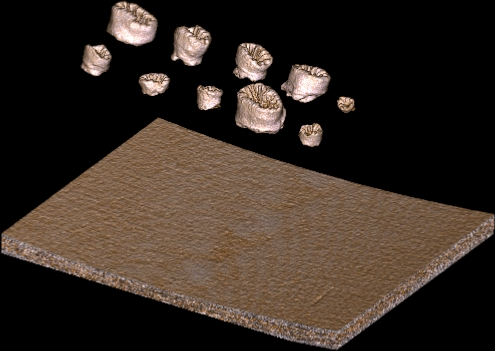
\includegraphics[scale=0.4]{Batches.jpg}
\caption{Batch of corals grown in non-acidified water}
\label{fig:1}
\end{figure}

\subsection{CT-Scan Information}

\

Our coral data consists of a sequence of DICOM files, a standard for handling, storing, printing and transmitting information in medical imaging. Each file contains information about a 2D slice of the coral, respresented as voxels that are characterized by a location in the 3D space and a density value. Voxels correspond to a real-life size of $0.199219 \times 0.199219 \times 0.199952$ mm$^3$, with density values ranging from -1024 to approx. 3000.

\

\section{Visualization Pipeline}

\

Cropping the independent coral samples from the two batches in DICOM format is the first step done for the purpose of visualization. To do this, we use the algorithm [TO BE ADDED BY TOBY AND ROBRECHT] and produce 20 VTI files, a file type which stores the 3D model of each coral sample.

\

Once the independent samples are cropped, we can analyze the effects that an acidified environment has on calcification by computing the \emph{density histogram}. The shape of the histogram can be used to infer the range of calcium carbonate density, but also its frequency. Several out-of-the-box tools such can be used for this purpose, such as ParaView\footnote{http://www.paraview.org/} or VolView\footnote{http://www.kitware.com/opensource/volview.html}.

\

A much more flexible approach to this is to use the open-source VTK\footnote{http://www.vtk.org/} visualization library and the Python\footnote{http://www.python.org/} scripting language. In our framework, we use the {\bf vtkXMLImageDataReader} class to read the contents of the VTI files and the 

\

\section{Evaluation of methods}
volume estimation with cubes, surfaces and integrating the density histogram. They give similar results but are different to the measured volume. counting the voxels is computational to expensive with VTK.
compare with measured volumes:
they differ because there is some massa which is not seen in the CT scan OR there are empty spaces in the coral which is also taken into account while measuring the volume

\section{Results}
values from -1000 to 2100(later)
show visualisations
show density graphs
compare with measured(real) values
\section{Conclusion}


\end{document}
